\part{2's Complement}
\frame{\partpage}

\begin{frame}{Modular arithmetic}
    \begin{columns}
        \begin{column}{0.4\textwidth}
            \begin{center}
                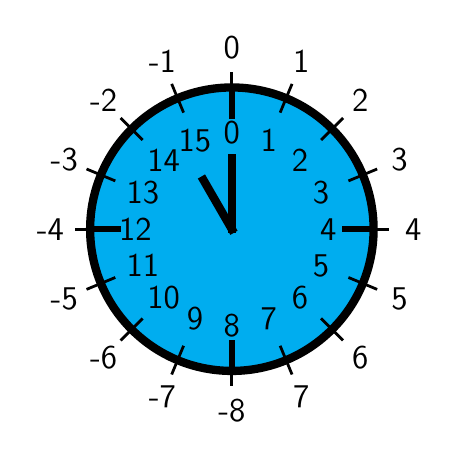
\begin{tikzpicture}[line cap=rect,line width=3pt,scale=0.9]
                    \filldraw [fill=cyan] (0,0) circle [radius=2cm];
                    \foreach \angle [count=\xi from 0] in {90,67.5,...,-247.5}
                    {
                        \draw[line width=1pt] (\angle:1.8cm) -- (\angle:2.2cm);
                        \node[font=\large] at (\angle:1.36cm) {\textsf{\xi}};
                    }
                    \foreach \angle [count=\xi from -8] in {270,247.5,...,-67.5}
                    {
                        \node[font=\large] at (\angle:2.56cm) {\textsf{\xi}};
                    }
                    \foreach \angle in {0,90,180,270}
                        \draw[line width=2pt] (\angle:1.6cm) -- (\angle:2cm);
                    \draw (0,0) -- (120:0.8cm);
                    \draw (0,0) -- (90:1cm);
                \end{tikzpicture}
            \end{center}
        \end{column}
        \begin{column}{0.55\textwidth}
            \begin{itemize}
                \pause\item Arithmetic \textbf{modulo} $N$
                \pause\item Numbers ``wrap around'' between $0$ and $N-1$
                \pause\item E.g.\ modulo $16$:
                    \begin{itemize}
                        \pause\item $14 + 7 = 5$
                        \pause\item $4 - 7 = 13$
                    \end{itemize}
            \end{itemize}
        \end{column}
    \end{columns}
\end{frame}

\begin{frame}{Modulo operator}
    \begin{itemize}
        \pause\item Present in many programming languages (including C++, C\#, Python) as \lstinline{\%}
        \pause\item \lstinline{a \% b} gives the \textbf{remainder} of \lstinline{a} divided by \lstinline{b}
        \pause\item E.g.\ \lstinline{21 \% 16} gives 5
        \pause\item Useful for wrapping around e.g.\ loop indexes or screen coordinates
    \end{itemize}
\end{frame}

\begin{frame}{2's complement}
    \begin{itemize}
        \pause\item How can we represent negative numbers in binary?
        \pause\item Represent them modulo $2^n$ (for $n$ bits)
        \pause\item I.e.\ represent $-a$ as $2^n-a$
        \pause\item Instead of an $n$-bit number ranging from $0$ to $2^n-1$, it ranges from $-2^{n-1}$ to $+2^{n-1}-1$
        \pause\item E.g.\ 16-bit number ranges from $-32768$ to $+32767$
        \pause\item Note that the left-most bit can be interpreted as a \textbf{sign} bit:
            $1$ if negative, $0$ if positive or zero
    \end{itemize}
\end{frame}

\begin{frame}{Converting to 2's complement}
    \begin{itemize}
        \pause\item Convert the absolute value to binary
        \pause\item Invert all the bits (i.e.\ change $0 \leftrightarrow 1$)
        \pause\item Add 1
        \pause\item (This is equivalent to subtracting the number from $2^n$... why?)
        \pause\item This is also the process for converting back from 2's complement,
            i.e.\ doing it twice should give the original number
    \end{itemize}
\end{frame}

\begin{frame}{Why 2's complement?}
    \begin{itemize}
        \pause\item Allows all addition and subtraction to be carried out modulo $2^n$
            without caring whether numbers are positive or negative
        \pause\item In fact, subtraction can just be done as addition
        \pause\item I.e.\ $a-b$ is the same as $a+(-b)$, where $a$ and $-b$ are just $n$-bit numbers
    \end{itemize}
\end{frame}
